\documentclass[aspectratio=1610]{beamer}

\usepackage{graphicx}
\usepackage[english]{babel}
\usepackage[T1]{fontenc}
\usepackage{csquotes, xcolor, xspace, changepage, setspace, listings}
\usepackage{libertinus}
\usepackage{roboto}
\usepackage{fontawesome5}
\usepackage[scale = 0.75]{plex-mono}
\usepackage{tikz, subcaption}

\usetikzlibrary{fit, shapes.geometric, shapes.symbols, positioning, shapes.misc, calc, arrows.meta, patterns, backgrounds, decorations, decorations.markings, decorations.pathreplacing, shadows, hobby}

\usepackage[backend=bibtex,style=authoryear]{biblatex}
\addbibresource{biblio.bib}

\title{3D Human Pose Tracking \\ using Multi-View 2D Detections}
\author{Roland Bernard}
\date{June 2026}

\definecolor{unibzblue}{HTML}{0086ec}
\definecolor{unibzblue2}{HTML}{f0f8ff}

\setbeamercolor{outerbox}{fg=black,bg=unibzblue2}
\setbeamercolor{innerbox}{fg=white,bg=unibzblue}

\setbeamertemplate{title page}{
  \scriptsize 
  \begin{tabular}{ll}
    \vspace*{40mm} \\
    \multicolumn{2}{l}{\raggedright Project Presentation -- Computer Vision 2025/2026} \\
    \\
    \multicolumn{2}{p{\linewidth}}{\raggedright \huge \bf \inserttitle} \\
    \\
    \\
    & \insertauthor \\
    \\
    & \insertdate \\
  \end{tabular}
}

\setbeamertemplate{frametitle}{
  \vspace*{6mm}
  \Large \bf \color{black} \insertframetitle
}

\setbeamertemplate{itemize items}{\scriptsize\raisebox{0.6mm}{\color{unibzblue} $\blacktriangleright$}}

\beamertemplatenavigationsymbolsempty
\setbeamertemplate{footline}{
  \begin{beamercolorbox}[wd=\paperwidth,right]{section in head/foot}
    \usebeamerfont{date in head/foot}\hspace*{2em}
    \insertframenumber{}\hspace*{2mm} 
    \vspace*{2mm}
  \end{beamercolorbox}
}

\newcommand{\litem}{{\scriptsize\raisebox{0.6mm}{\color{unibzblue} $\blacktriangleright$}}}
\newcommand{\sitem}{{\scriptsize\raisebox{0.2mm}{\color{unibzblue} $\rightarrow$}}\enspace}
\newcommand{\icon}[1]{\textcolor{unibzblue}{\faIcon[solid]{#1}}}

\newlength{\offsetpage}
\newenvironment{narrowpage}[1][3mm]{
  \setlength{\offsetpage}{#1}
  \begin{adjustwidth}{\offsetpage}{\offsetpage}
}{
  \end{adjustwidth}
}
\newenvironment{widepage}[1][10mm]{
  \setlength{\offsetpage}{#1}
  \begin{adjustwidth}{-\offsetpage}{-\offsetpage}
}{
  \end{adjustwidth}
}

\newenvironment{items}{
  \begin{narrowpage}
}{
  \end{narrowpage}
}
\newenvironment{oitem}[2][3mm]{
  \vspace*{2mm}
  \begin{beamercolorbox}[rounded=false,colsep=#1]{outerbox}
    \parbox[t]{2mm}{\centering#2}\parbox[t]{2mm}{\ }%
    \begin{minipage}[t]{\linewidth}
}{
    \end{minipage}
  \end{beamercolorbox}
  \vfill
}

\definecolor{unibzblue}{HTML}{0086ec}
\definecolor{unibzblue2}{HTML}{f0f8ff}

\pgfdeclarelayer{background}
\pgfdeclarelayer{foreground}
\pgfsetlayers{background,main,foreground}

\definecolor{input}{HTML}{b2e684}
\definecolor{parameter}{HTML}{e38e48}
\definecolor{compute}{HTML}{df7162}

\tikzset{
  flow/.style={-{Triangle[length=4, width=4]}, draw=red!70!black, thick, shorten >= -1},
  biflow/.style={flow, {Triangle[length=6, width=6]}-{Triangle[length=6, width=6]}},
  link/.style={->, draw},
  ptr/.style={->, dashed},
  leafl/.style={-, thick},
  external/.style={draw=black, fill=brown!20},
  internal/.style={inner sep=10, draw=black, fill=unibzblue!20},
  build/.style={inner sep=10, draw=black, fill=unibzblue!40},
  mixed/.style={inner sep=8.7, draw=black, path picture={
    \fill[brown!20] (path picture bounding box.south west)
      rectangle ($(path picture bounding box.north west)!.675!(path picture bounding box.north east)$);
    \fill[unibzblue!40] ($(path picture bounding box.north west)!.675!(path picture bounding box.north east)$)
      rectangle (path picture bounding box.south east);
  }},
  block/.style={rounded corners, draw=unibzblue, fill=unibzblue2, thick, 
      minimum width=15mm, minimum height=5mm, align=center, inner sep=2},
  small/.style={circle, draw=purple!60, fill=purple!20, thick, 
      minimum width=3mm, minimum height=3mm, align=center},
  conv/.style={rectangle, draw=blue!60, fill=blue!20, thick, 
      minimum width=15mm, minimum height=5mm, align=center, inner sep=2},
  op/.style={rounded corners, draw=green!60, fill=green!20, thick, 
      minimum width=13mm, minimum height=5mm, align=center, inner sep=2},
  pool/.style={rectangle, draw=red!60, fill=red!20, thick, 
      minimum width=15mm, minimum height=5mm, align=center, inner sep=2},
  dropout/.style={rectangle, draw=gray!60, fill=gray!20, thick, 
      minimum width=12mm, minimum height=5mm, align=center, inner sep=2},
  base_node/.style={minimum height=5mm,align=center,text width=20mm},
  icon_node/.style={minimum size=7mm,align=center}
  >=Latex, node distance=1, every node/.style={font=\footnotesize, inner sep=0}
}


\begin{document}

\begin{frame}[plain]
  \begin{tikzpicture}[
    remember picture, overlay,
    every path/.style={opacity=0.10},
    yshift=20, xshift=200, scale=1.5, transform shape
  ]
    \node {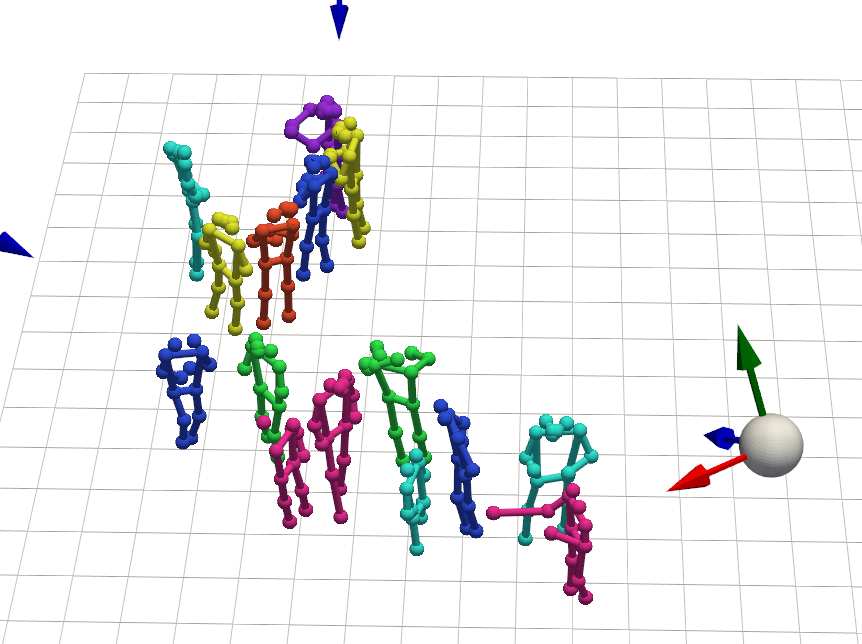
\includegraphics[width=0.9\linewidth]{figures/background.png}};
  \end{tikzpicture}
  \titlepage
\end{frame}

\begin{frame}
\frametitle{Introduction}
  \begin{items}
    \begin{oitem}{\litem}
      Problem: {\footnotesize Multiple video sequences containing multiple people.}
    \end{oitem}
    \begin{oitem}{\litem}
      Possible Applications: \\
      {\footnotesize Multiple video sequences containing multiple people.} \\
      {\footnotesize Multiple video sequences containing multiple people.} \\
      {\footnotesize Multiple video sequences containing multiple people.}
    \end{oitem}
    \begin{oitem}{\litem}
      Task Formulation: \\
      \sitem {\footnotesize 3D coordinates of skeletal joint for each subject.} \\
      \sitem {\footnotesize 3D coordinates of skeletal joint for each subject.} \\
      \sitem {\footnotesize 3D coordinates of skeletal joint for each subject.} \\
      \sitem {\footnotesize Movement of skeletal joint over time.}
    \end{oitem}
    \vspace*{2mm}
    \begin{figure}
      \centering
      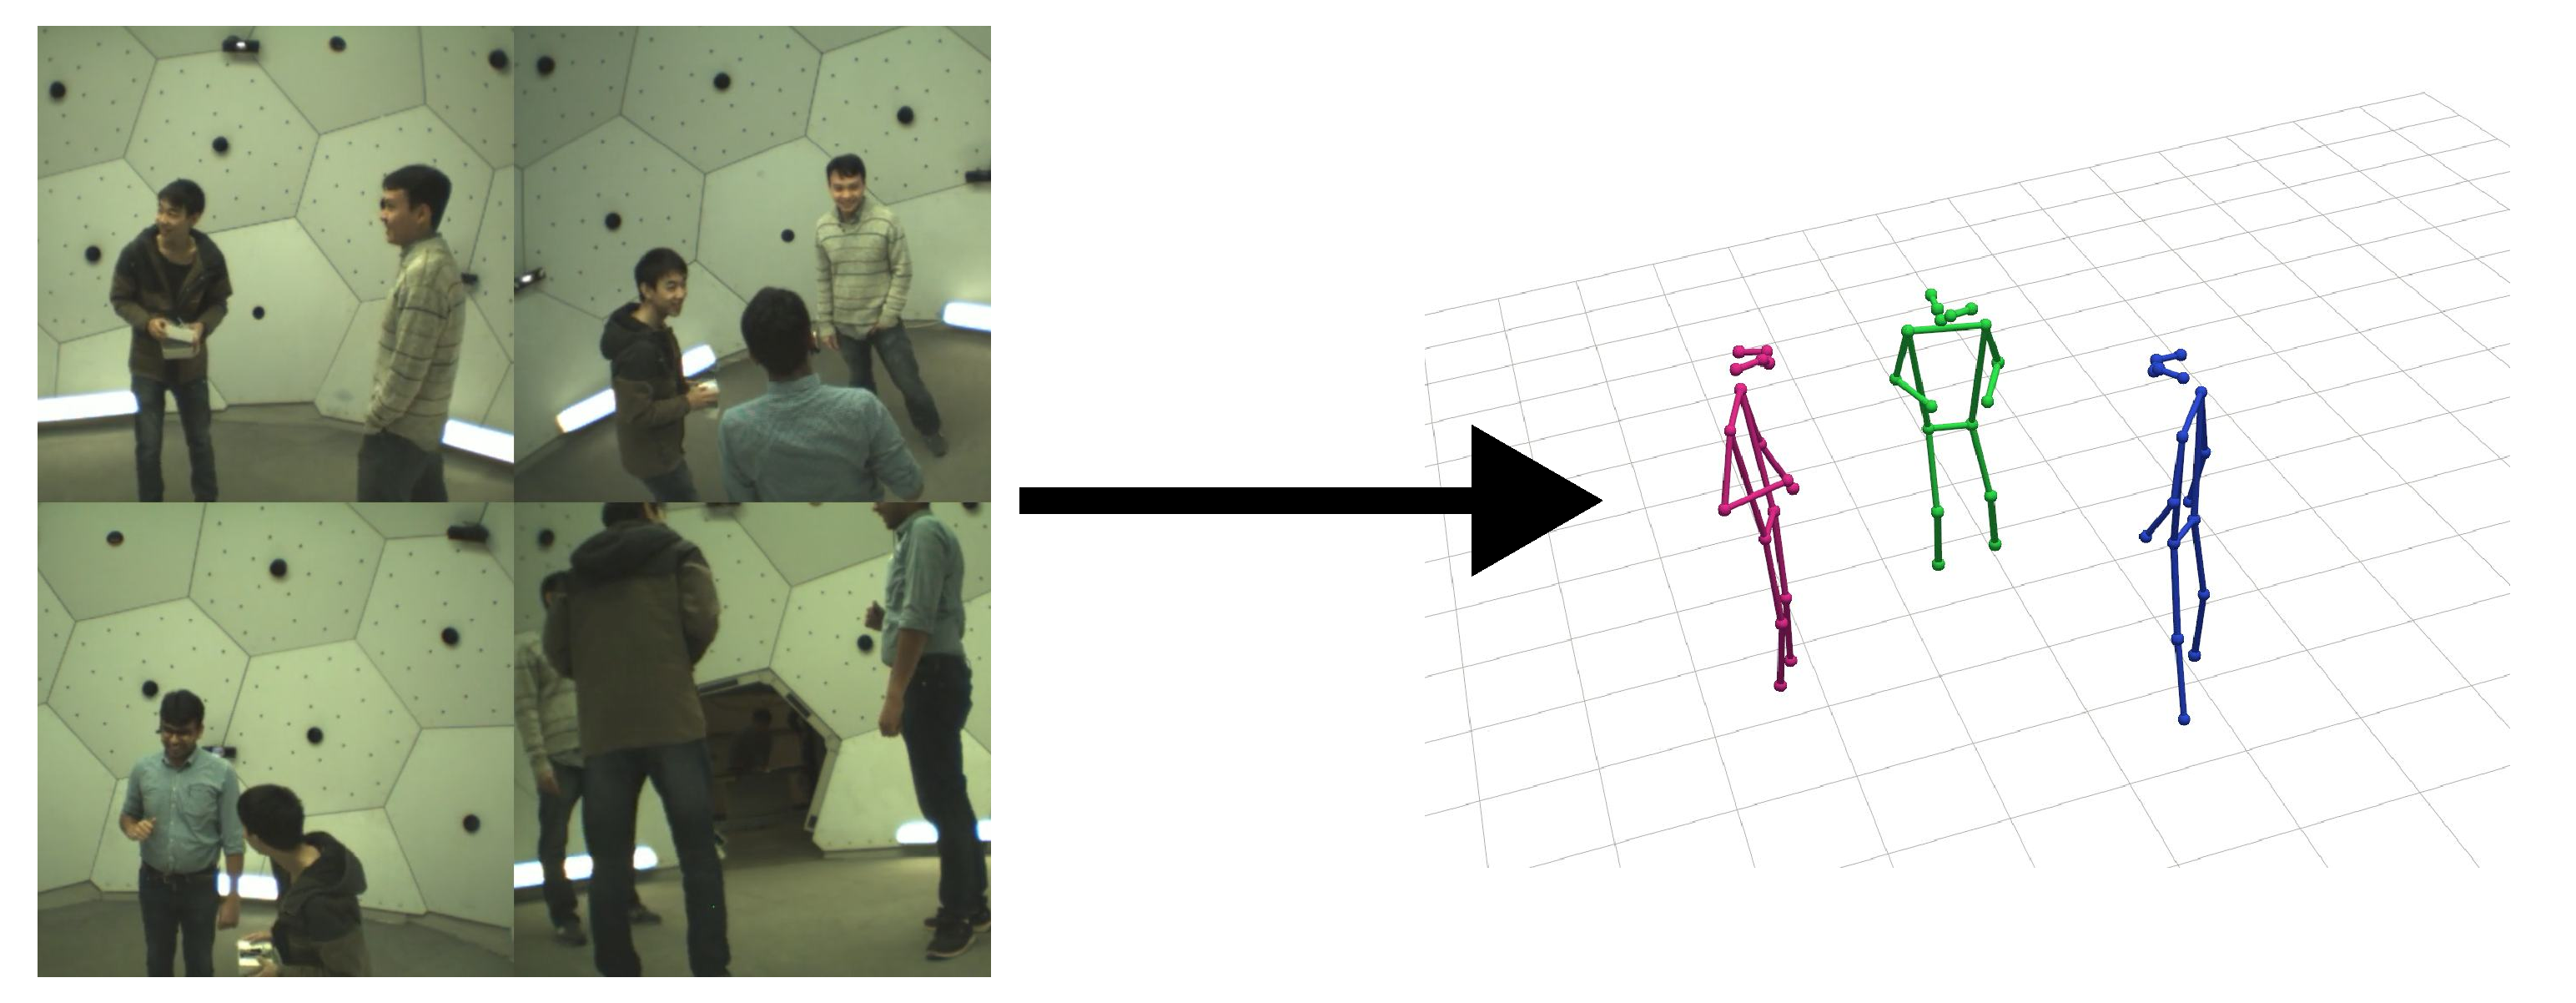
\includegraphics[width=0.9\linewidth]{figures/introduction.pdf}
    \end{figure}
  \end{items}
\end{frame}

\begin{frame}
\frametitle{Task Formulation}
  \begin{items}
    \begin{oitem}{\litem}
      Given: {\footnotesize Multiple video sequences containing multiple people.}
    \end{oitem}
    \begin{oitem}{\litem}
      Output: \\
      {\footnotesize Multiple video sequences containing multiple people.} \\
      {\footnotesize Multiple video sequences containing multiple people.} \\
      {\footnotesize Multiple video sequences containing multiple people.}
    \end{oitem}
    \vspace*{2mm}
    \begin{figure}
      \centering
      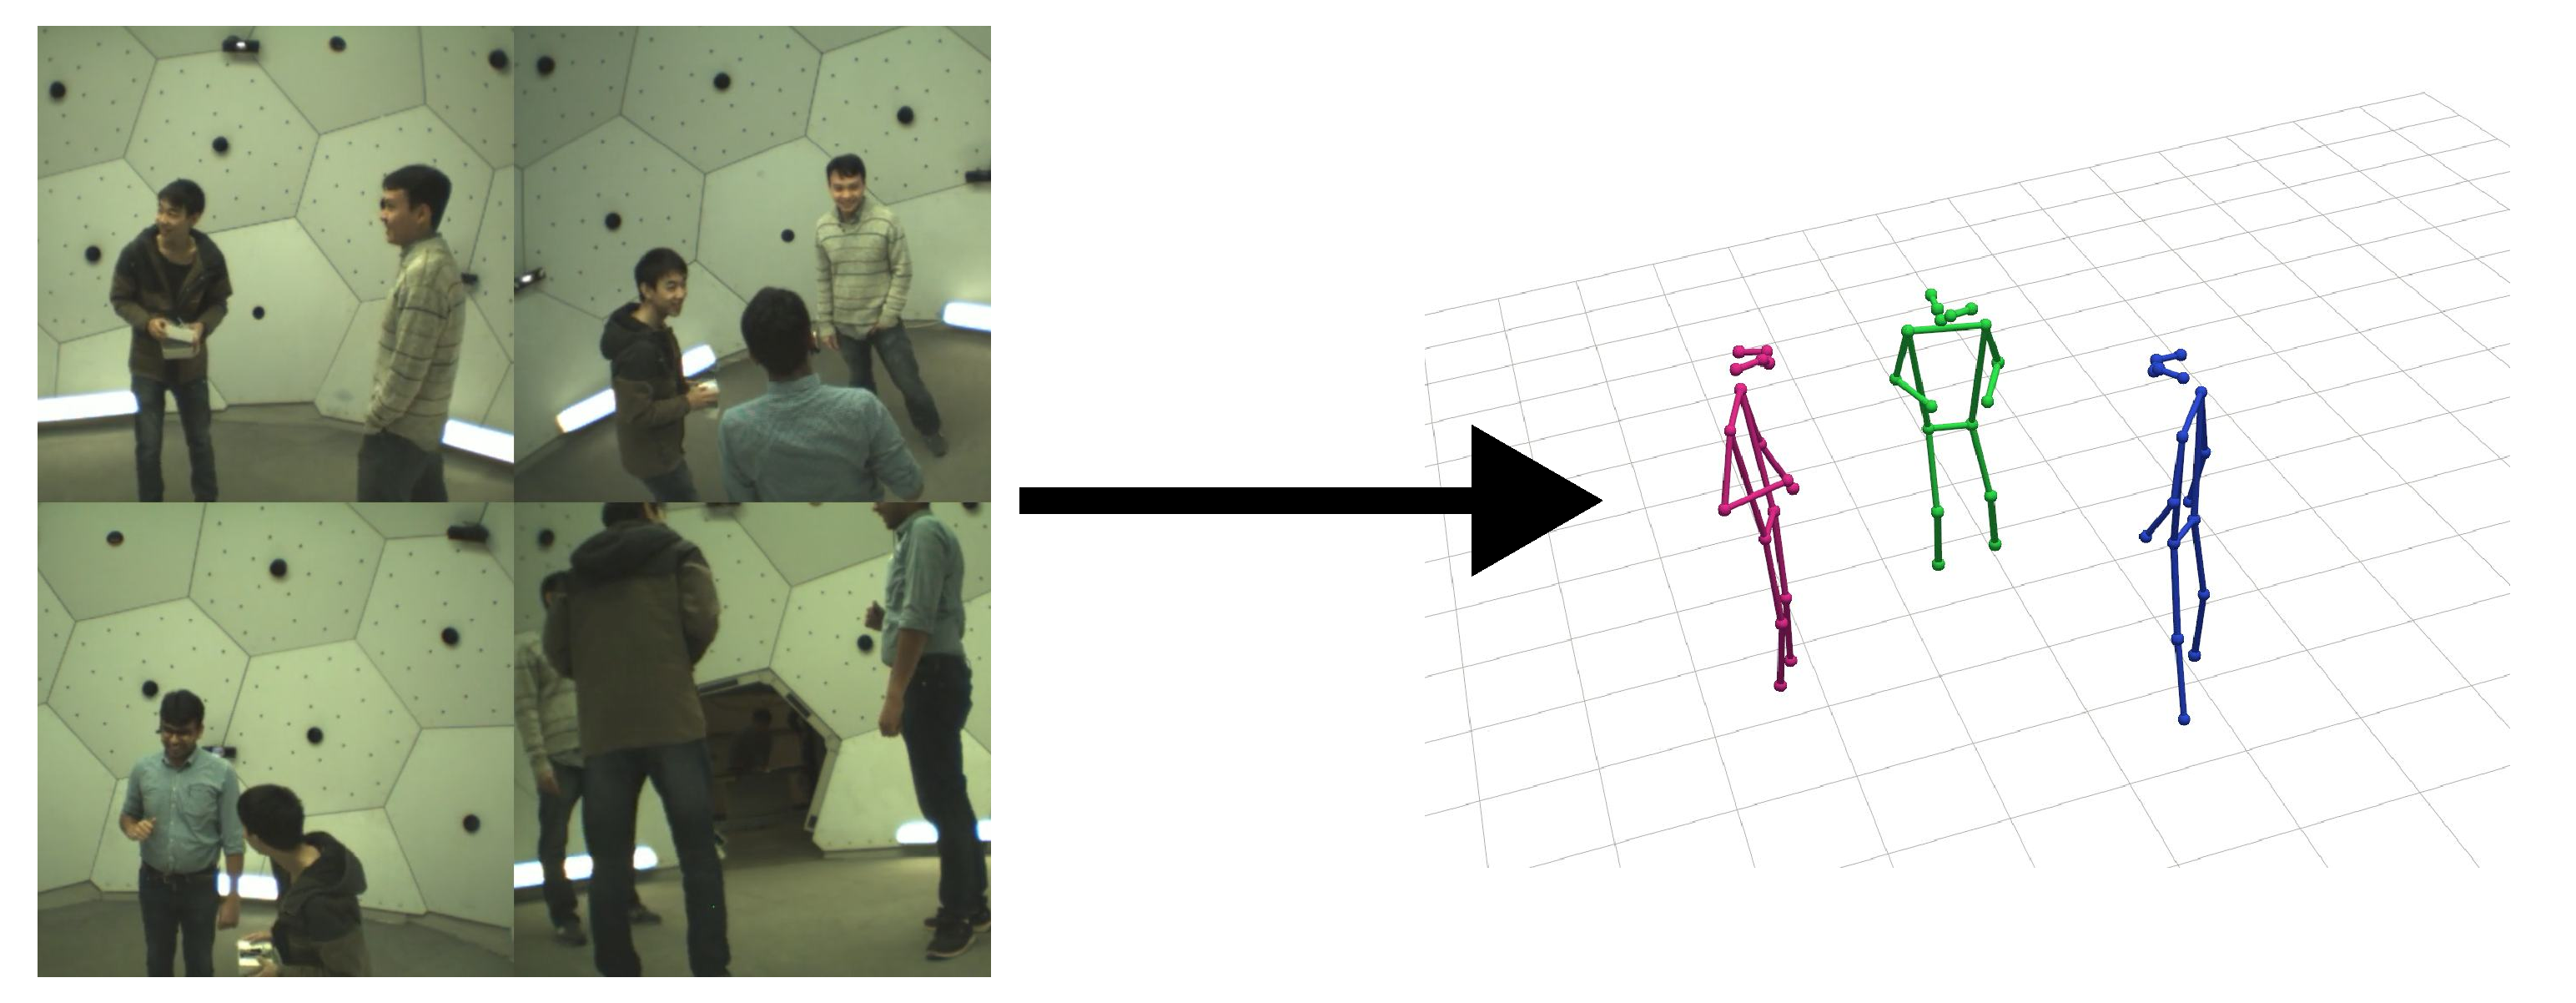
\includegraphics[width=0.9\linewidth]{figures/introduction.pdf}
    \end{figure}
  \end{items}
\end{frame}

\begin{frame}
\frametitle{System Architecture -- Overview}
  \begin{items}
    \begin{oitem}{\litem}
      Summary: \\
      \sitem {\footnotesize Perform single-view single-frame 2D estimation using pretrained model.} \\
      \sitem {\footnotesize Reconstruct 3D geometry from multiple camera views via triangulation.}
    \end{oitem}
  \end{items}
\end{frame}

\begin{frame}
\frametitle{System Architecture -- 2D Detections}
  \begin{items}
    \begin{oitem}{\litem}
      Summary: \\
      \sitem {\footnotesize Perform single-view single-frame 2D estimation using pretrained model.} \\
      \sitem {\footnotesize Reconstruct 3D geometry from multiple camera views via triangulation.}
    \end{oitem}
  \end{items}
\end{frame}

\begin{frame}
\frametitle{System Architecture -- Kalman Filtering}
  \begin{items}
    \begin{oitem}{\litem}
      Summary: \\
      \sitem {\footnotesize Perform single-view single-frame 2D estimation using pretrained model.} \\
      \sitem {\footnotesize Reconstruct 3D geometry from multiple camera views via triangulation.}
    \end{oitem}
  \end{items}
\end{frame}

\begin{frame}
\frametitle{System Architecture -- Data Association}
  \begin{items}
    \begin{oitem}{\litem}
      Summary: \\
      \sitem {\footnotesize Perform single-view single-frame 2D estimation using pretrained model.} \\
      \sitem {\footnotesize Reconstruct 3D geometry from multiple camera views via triangulation.}
    \end{oitem}
  \end{items}
\end{frame}

\begin{frame}
\frametitle{Dataset Overview}
  \begin{items}
    \begin{oitem}{\litem}
      Source:: \\
      \sitem {\footnotesize Perform single-view single-frame 2D estimation using pretrained model.} \\
      \sitem {\footnotesize Reconstruct 3D geometry from multiple camera views via triangulation.}
    \end{oitem}
    \begin{oitem}{\litem}
      Format and Data Characteristics: \\
      \sitem {\footnotesize Perform single-view single-frame 2D estimation using pretrained model.} \\
      \sitem {\footnotesize Reconstruct 3D geometry from multiple camera views via triangulation.} \\
      \sitem {\footnotesize Apply Kalman filtering to smooth out noise.}
    \end{oitem}
  \end{items}
\end{frame}

\begin{frame}
\frametitle{Experimental Setup}
  \begin{items}
    \begin{oitem}{\litem}
      Setup: \\
      \sitem {\footnotesize Perform single-view single-frame 2D estimation using pretrained model.} \\
      \sitem {\footnotesize Reconstruct 3D geometry from multiple camera views via triangulation.} \\
      \sitem {\footnotesize Apply Kalman filtering to smooth out noise.}
    \end{oitem}
    \begin{oitem}{\litem}
      Evaluation Metrics: \\
      \sitem {\footnotesize Perform single-view single-frame 2D estimation using pretrained model.} \\
      \sitem {\footnotesize Reconstruct 3D geometry from multiple camera views via triangulation.} \\
      \sitem {\footnotesize Apply Kalman filtering to smooth out noise.}
    \end{oitem}
  \end{items}
\end{frame}

\begin{frame}
\frametitle{Quantitative Results -- Runtime Efficiency}
  \begin{items}
    \begin{oitem}{\litem}
      Main Finding: \\
      \sitem {\footnotesize Occlusions can make some joints unobserved.} \\
      \sitem {\footnotesize Matching predictions between multiple views.} \\
      \sitem {\footnotesize Matching predictions across time.}
    \end{oitem}
    \begin{figure}
      \centering
      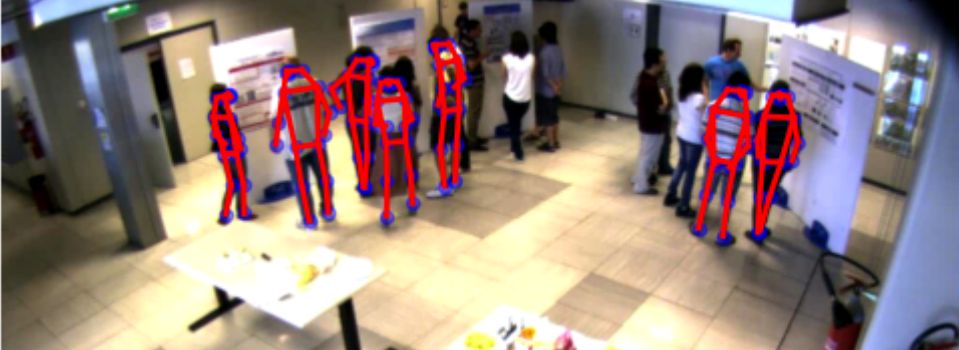
\includegraphics[width=\linewidth]{figures/difficulties.png}
    \end{figure}
  \end{items}
\end{frame}

\begin{frame}
\frametitle{Quantitative Results -- Performance vs. Model Size}
  \begin{items}
    \begin{oitem}{\litem}
      Main Finding: \\
      \sitem {\footnotesize Occlusions can make some joints unobserved.} \\
      \sitem {\footnotesize Matching predictions between multiple views.} \\
      \sitem {\footnotesize Matching predictions across time.}
    \end{oitem}
    \begin{figure}
      \centering
      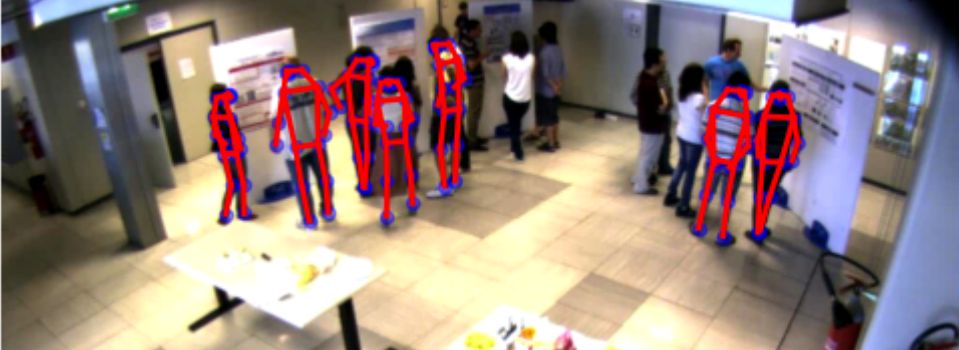
\includegraphics[width=\linewidth]{figures/difficulties.png}
    \end{figure}
  \end{items}
\end{frame}

\begin{frame}
\frametitle{Quantitative Results -- Performance vs. Camera Count}
  \begin{items}
    \begin{oitem}{\litem}
      Main Finding: \\
      \sitem {\footnotesize Occlusions can make some joints unobserved.} \\
      \sitem {\footnotesize Matching predictions between multiple views.} \\
      \sitem {\footnotesize Matching predictions across time.}
    \end{oitem}
    \begin{figure}
      \centering
      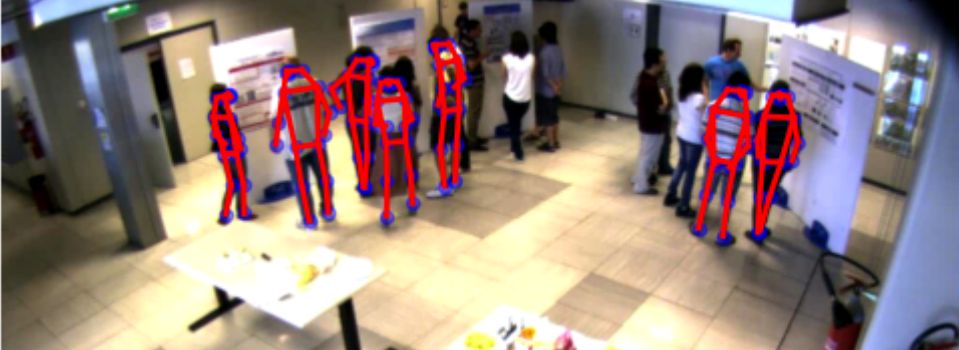
\includegraphics[width=\linewidth]{figures/difficulties.png}
    \end{figure}
  \end{items}
\end{frame}

\begin{frame}
\frametitle{Qualitative Results}
  \begin{items}
    \begin{oitem}{\litem}
      Visual Observations: \\
      \sitem {\footnotesize Keep internal 3D state of all currently tracked persons.} \\
      {\footnotesize Repeat for each frame:} \\
      \sitem {\footnotesize Predict next frame state using current state.} \\
      \sitem {\footnotesize Match predictions with detections.}
    \end{oitem}
    \begin{figure}
      \centering
      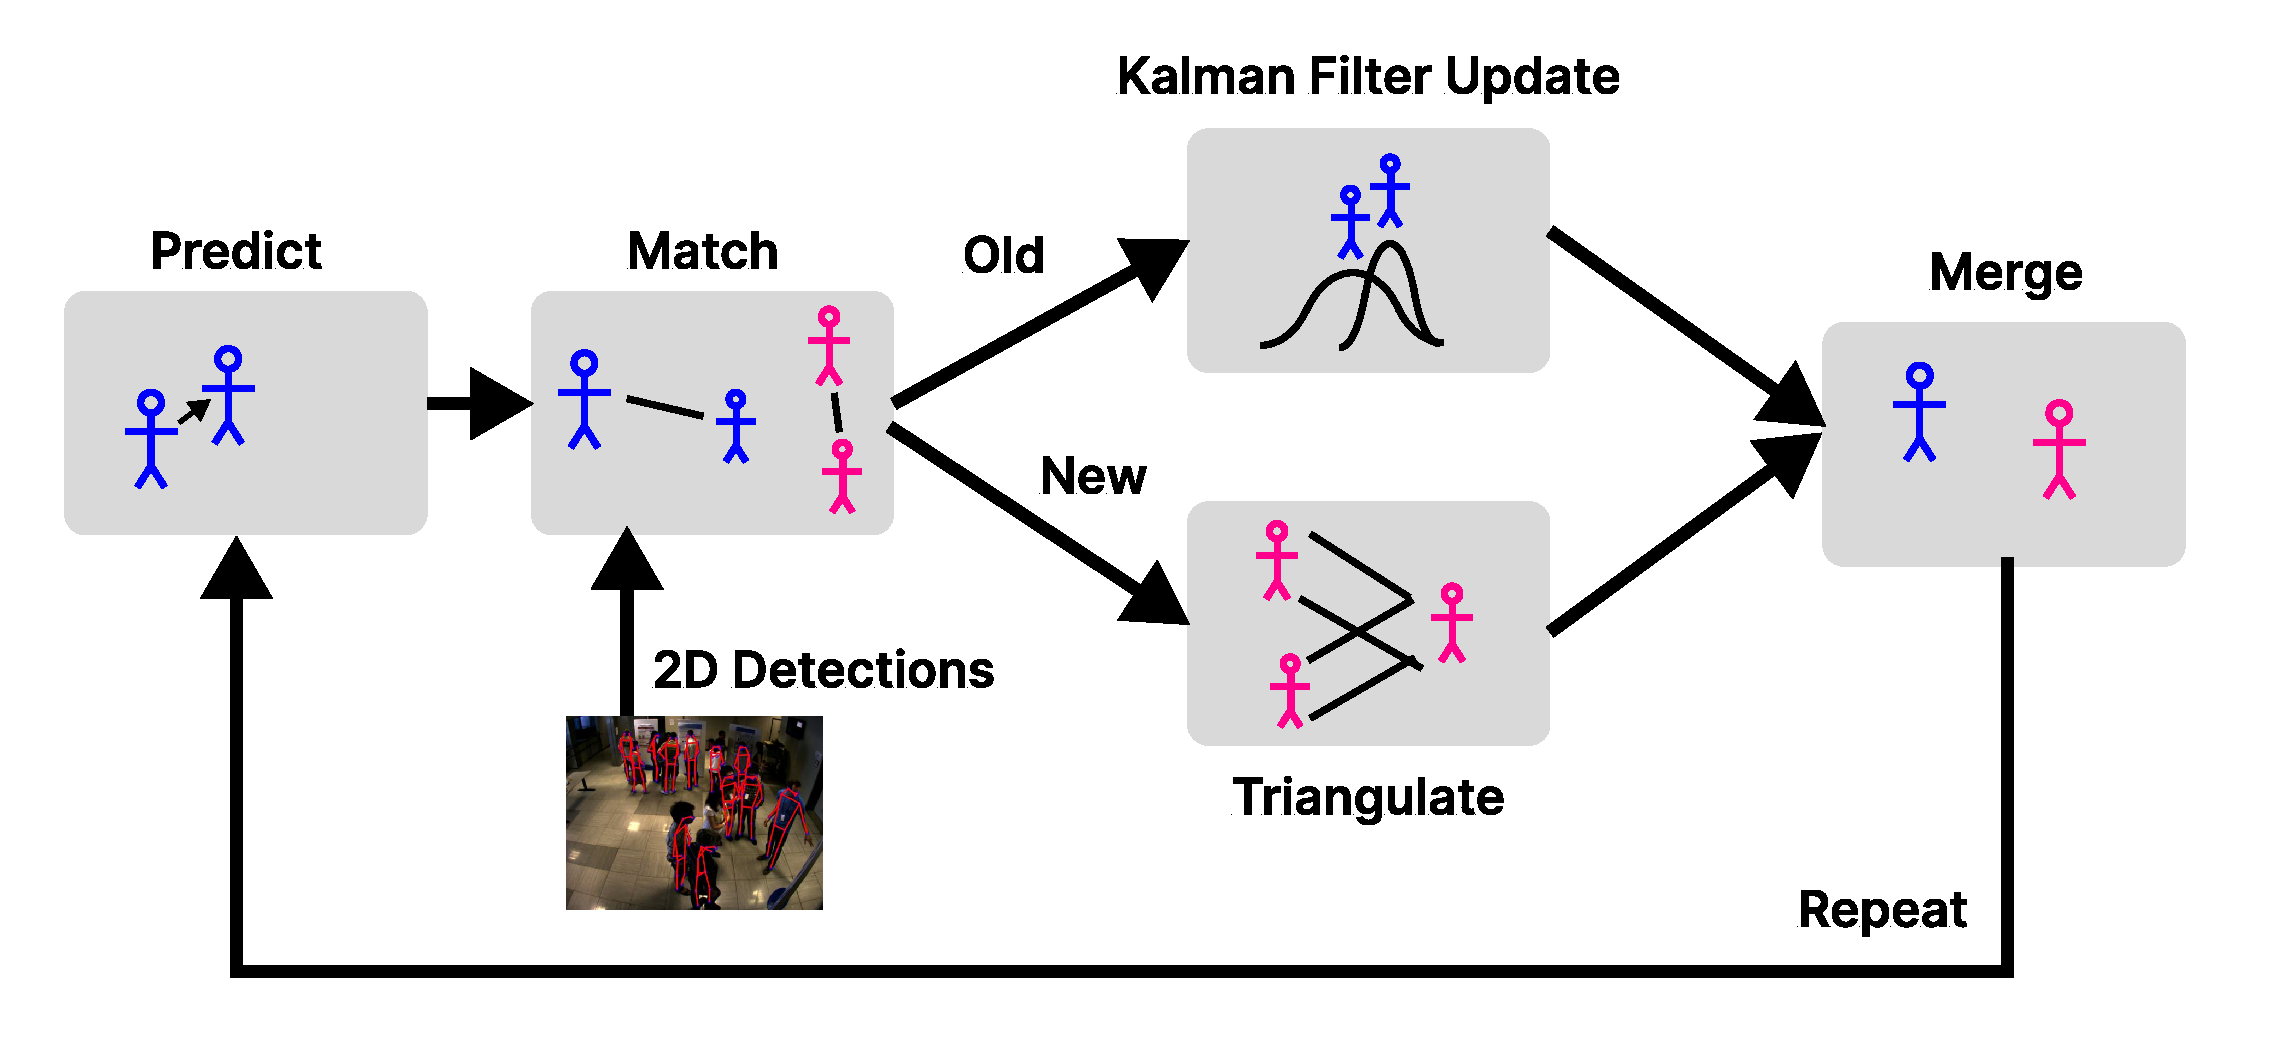
\includegraphics[width=0.7\linewidth]{figures/kalman.pdf}
    \end{figure}
  \end{items}
\end{frame}

\begin{frame}
\frametitle{Conclusion}
  \begin{items}
    \begin{oitem}{\litem}
      Summary: \\
      \sitem {\footnotesize Implemented an EKF framework that merges multi-view observations.} \\
      \sitem {\footnotesize Analyzed performance across different model sizes and camera densities.}
    \end{oitem}
    \begin{oitem}{\litem}
      Limitations: \\
      \sitem {\footnotesize Struggles significantly with occlusions.} \\
      \sitem {\footnotesize Running 2D pose estimation on every camera view remains a performance bottleneck.}
    \end{oitem}
    \begin{oitem}{\litem}
      Possible Future Improvements: \\
      \sitem {\footnotesize Data-driven learning filter parameters.} \\
      \sitem {\footnotesize Add constraints that force anatomical consistency of joints.}\\
      \sitem {\footnotesize Fine-tuning of the 2D pose estimation model.} \\
      \sitem {\footnotesize Integration of monocular depth estimation.} \\
      \sitem {\footnotesize Use of a particle filter with occlusion aware likelihood.}
    \end{oitem}
  \end{items}
\end{frame}


{
\setbeamercolor{background canvas}{bg=black}
\begin{frame}[plain]{}
\end{frame}
}

\end{document}
